\section{Umsetzung}
\label{sec:umsetzung}

Bevor die genauen Durchführungen der einzelnen Doppelstunden betrachtet werden, sind zunächst einige Vorbemerkungen zu machen.

Erstens waren die folgenden selbst gehaltenen Stunden nicht das erste Kennenlernen der Klasse.
Zuvor wurden bereits beide Hälften während Hospitationen bei Unterrichtsstunden zum Thema Python besucht und kennen gelernt.
Währenddessen konnten auch erste Beobachtungen bezüglich der sozialen und persönlichen Verhältnisse der Schülerinnen und Schüler gemacht werden, welche in die in \autoref{sec:konzeption} getroffene Konzeption des Unterrichts mit einfließen konnten.

Weiterhin war es nötig, dass die Klasse im eingeplanten Zeitraum eine Klassenarbeit schreiben musste, in welcher die in der vorhergehenden Unterrichtseinheit behandelten Inhalte (hauptsächlich Programmierung in Python) abgefragt werden würde.
Ein großer Nachteil davon war, dass die folgende Unterrichtseinheit durch eine Doppelstunde unterbrochen werden würde, in welcher die Arbeit geschrieben wurde.
Leider war es nicht möglich, den Termin anders zu legen, weswegen diese Unterbrechung mit in die Planung aufgenommen wurde.


\subsection{Erste Doppelstunde}
\label{subsec:doppelstunde-1}

Der Einstieg in den Unterricht erfolgte problemorientiert anhand eines Beispiels.
Gezeigt wurde eine Webseite, auf der die mit HTML und CSS gestaltete Eingabemaske eines Promillerechners zu sehen war.
Ein Ausschnitt der genannten Webseite ist in \autoref{fig:promillerechner} abgebildet.

\begin{figure}[h!]
	\centering
	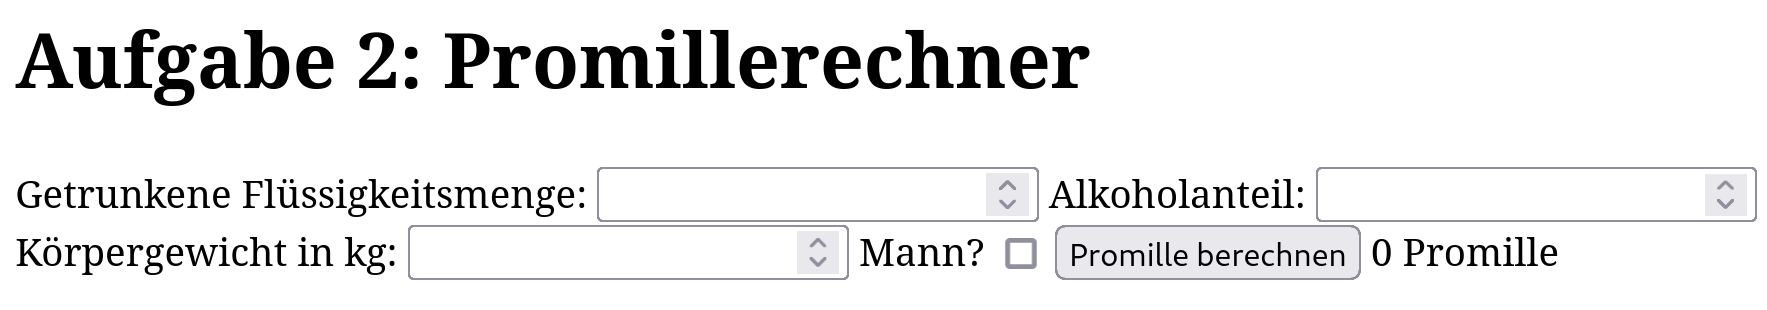
\includegraphics[width=\textwidth]{media/Promillerechner.png}
	\caption{Webseite des Promillerechners}
	\label{fig:promillerechner}
\end{figure}

Bei Nutzung der Webseite wurde demonstriert, dass diese keinerlei Funktion hatte.
Ein großes Ziel der ersten Doppelstunde war, den aktuellen Vorwissensstand der Schülerinnen und Schüler zum Thema Webentwicklung herauszufinden.
Die präsentierte Webseite wurde so einerseits dazu genutzt, um den Schülerinnen und Schüler einen Ausblick auf die kommenden Stunden zu geben und ihnen klar zu machen, dass wir uns nun (wieder) mit dem Thema Webentwicklung beschäftigen.
Andererseits wurde damit auch eine Diskussion darüber angestoßen, aus was eine Webseite denn besteht und woran sie sich noch erinnern können.
An dieser beteiligten sich die Schülerinnen und Schüler sehr engagiert und es fielen auch Fachbegriffe wie HTML.
Auf Nachfrage wurde jedoch schnell ersichtlich, dass nur wenig Wissen über das Thema HTML vorhanden war.

Dies wurde als Überleitung zum ersten Arbeitsblatt genutzt, welches in \autoref{pdf:ab_html_css} zu sehen ist.
Das Übungsblatt sollte zunächst in Einzelarbeit bearbeitet werden, bei Schwierigkeiten konnten die Schülerinnen und Schüler jedoch selbstständig zur Partnerarbeit übergehen.
In der Besprechung des Blatts wurde schnell klar, dass die meisten Fragen nur durch Internetrecherche beantwortet werden konnten und viele der Lerninhalte aus der Einheit zu HTML nicht mehr präsent waren.
Mit CSS konnte nur ein Schüler etwas anfangen, die anderen hatten noch nie davon gehört.
Während dies für die Schülerinnen und Schüler frustrierend gewirkt haben kann, war es dennoch ein wichtiges Vorgehen.
Nun war klar, dass die kommenden Stunden nicht auf Dinge aufbauen konnten, die über ein Grundwissen von HTML hinausgingen und kein bzw. nur sehr grundlegendes CSS verwendet werden konnte.

Die anschließende Erklärung der Syntax von Javascript und ihren Aufbau als Programmiersprache verlief grundsätzlich produktiv.
Von den Schülerinnen und Schülern kamen nur wenige Fragen, jedoch wurde anschließend das in \autoref{pdf:merkblatt_variablen_if} stehende Merkblatt als sehr hilfreich erachtet.
Lediglich die für die kommenden Aufgaben notwendige Funktion \texttt{document.getElementById()} war schwierig zu verstehen.
Hier konnte die Verwendung durch zahlreiche Beispiele anhand der Nutzung der Funktion in der Konsole auf einer Webseite verdeutlicht werden.
Dennoch sollte dies ein Problem bleiben, welches dauerhaft bestehen blieb, was sich jedoch erst beim Feedback am Ende der Unterrichtseinheit herausstellte.

Die oben genannten Schwierigkeiten spiegelten sich auch in der Bearbeitung des folgenden Übungsblattes wider, welches sich in \autoref{pdf:ab_variablen_if} finden lässt.
Viele Schülerinnen und Schüler wussten nicht weiter.
Resultierend daraus mussten zusätzliche Erklärungen und Beispiele eingeschoben sowie die Bearbeitungszeit für das Blatt nach oben angepasst werden.
Schlussendlich hatte es niemand geschafft, über Aufgabe 2 hinauszukommen.
Die Konsequenz daraus war, dass die Planung für die nächste Stunde angepasst werden musste, um den Schülerinnen und Schüler dort genügend Zeit für die restlichen Aufgaben zu ermöglichen, da in diesen das essentielle Konzept der if-Verzweigung eingeübt wurde.

Die Durchführung der Stunde in der anderen Hälfte der Klasse war insofern anders, als dass bei der Planung dieser auf die Vorerfahrungen aus der ersten Durchführung in der anderen Klassenhälfte zurückgegriffen werden konnte.
Beispielsweise war schon im Vorhinein klar, dass eine Wiederholung der Inhalte zu CSS nicht notwendig oder sogar verwirrend und frustrierend für die Schülerinnen und Schüler war.
Entsprechend wurde auch das Übungsblatt zur Vorwissensreaktivierung angepasst; diese Version findet sich in \autoref{pdf:ab_html}.
Außerdem konnte davon ausgegangen werden, dass die Schülerinnen und Schüler für die Bearbeitung der Aufgaben mehr Zeit als geplant benötigten und vertiefende Erklärungen zur Funktion \texttt{document.getElementById()} notwendig waren.
Auch um den Teil der Klasse auf einem ähnlichen Stand zu halten wurde also weniger Stoff in der Doppelstunde behandelt, dafür jedoch mit ausführlicheren Erklärungen.

Angenommen wurde dies von der Klasse gut.
Auch hier traten Schwierigkeiten bei der Verwendung der oben genannten Funktion auf, jedoch konnten diese die vertieften Erklärungen sowie zahlreiche Beispiele weitestgehend ausgeglichen werden.
Grundsätzlich wirkte dieser Teil der Klasse generell motivierter für das Fach und arbeitete konzentriert mit.
Einen Einfluss darauf könnte die durch das Fehlen einiger Schülerinnen und Schüler bedingte geringere Gruppengröße gehabt haben, was eine individuellere Förderung in den Arbeitsphasen ermöglichte.


\subsection{Zweite Doppelstunde}
\label{subsec:doppelstunde-2}

Leider wurde der Start des Unterrichts aufgrund technischer Schwierigkeiten verzögert.
Die Verbindung des Computers mit dem Whiteboard schlug fehl, was den Unterricht unmöglich machte.
Da die betreuende Lehrkraft wegen ihrer Tätigkeit in der Schulleitung leider von einem Kollegen benötigt wurde und sie daher nicht vor Ort war, um bei der Beseitigung des Problems zu helfen, dauerte es 10 Minuten, bis der Unterricht regulär starten konnte.

Der Einstieg in die zweite Stunde erfolgte mit einem Kahoot \cite{wang2020kahoot, dellos2015kahoot}, in dem es um die bereits erlernte Syntax von Javascript ging.
Dabei wurden auch mögliche Fehlvorstellungen bzw. Verwechslungen mit der Syntax von Python-Code aufgegriffen.
Das Quiz wurde von den Schülerinnen und Schülern sehr gut angenommen und schien die Motivation für die kommende Stunde deutlich zu steigern.
Ebenfalls konnten so Verständnisschwierigkeiten, die vom letzten Mal noch bestanden, beseitigt werden, beispielsweise die Verwendung von geschweiften Klammern in Javascript statt einem Doppelpunkt in Python.

Aufgrund der Schwierigkeiten, die bereits in der ersten Doppelstunde bei den Schülerinnen und Schülern aufgetreten waren, war es nicht möglich, sämtliche für die erste Stunde vorgesehenen Aufgaben zu bearbeiten und zu besprechen.
Wie bereits erwähnt kam niemand über Aufgabe 2 hinaus, während in der Planung von drei bearbeiteten Aufgaben ausgegangen war.
Aufgabe 3 war dabei so gestaltet, dass eine Lösung sowohl durch if-Verzweigungen, als auch durch die Nutzung einer Liste möglich war.
Da die Aufgabe jedoch noch nicht bearbeitet worden war, war auch die Nutzung dieser Aufgabe als Heranführung an das neue Thema nicht möglich.
Infolgedessen musste die Planung der Stunde verändert werden, so dass erst nachgeholt werden konnte, was in der letzten Stunde nicht mehr geschafft worden war.

Während der zusätzlich eingeplanten Arbeitszeit stellte sich heraus, dass die Schülerinnen und Schüler noch deutlich mehr Zeit benötigten als ursprünglich eingeplant.
In der zusätzlich eingeplanten Arbeitsphase von 25 Minuten schaffte es niemand, die noch offene Aufgabe 3 fertig zu bearbeiten, insbesondere deshalb, da auch einige Schülerinnen und Schüler noch mit Aufgabe 2 beschäftigt waren.
Nach Rücksprache mit der Klasse wurde daraufhin entschieden, die Doppelstunde als weitere Übungsstunde zu nutzen und das Thema Listen erst in der kommenden Stunde anzufangen.
Einfluss auf diese Entscheidung hatten auch der verzögerte Start sowie die Aussage der Klasse, mehr Zeit und eine zusätzliche Erklärung wären sehr hilfreich.

Da nun die gesamte Doppelstunde dazu genutzt werden konnte, die Übungsaufgaben 2 und 3 fertig zu bearbeiten, war es sämtlichen Schülerinnen und Schülern möglich, dieses Ziel am Ende der Stunde zu erreichen.
Sehr positiv war dabei, dass sich die Schülerinnen und Schüler untereinander geholfen haben und die schnelleren die langsameren unterstützt haben.
Auch in der abschließenden Besprechung der Aufgaben kamen insbesondere zur Bildergalerie zahlreiche verschiedene Lösungsansätze.
Dies regte unter den Schülerinnen und Schülern weitere Diskussionen darüber an, welche der vorgestellten Lösungen die eleganteste und beste sei.

Vor diesem Hintergrund stellte sich nun die Frage, wie die entsprechende Stunde in der zweiten Hälfte der Klasse durchzuführen wäre.
Einerseits war es ungünstig, die beiden Hälften auf unterschiedlichem Stand zu unterrichten, allerdings war es auch nicht sinnvoll, eine Doppelstunde ungenutzt zu lassen und Übungen zur Verfügung zu stellen, obwohl eigentlich neuer Stoff hätte behandelt werden können.
Schlussendlich fiel die Entscheidung darauf, ebenfalls eine weitere Übungsstunde in der anderen Klassenhälfte durchzuführen und das Thema Listen noch um eine Woche zu verschieben.
Dies geschah aus mehreren Gründen:
\begin{itemize}
	\item Die betreuende Lehrkraft erkrankte leider, was Unterstützungsmöglichkeiten in fachlicher, aber auch technischer Hinsicht einschränkte.
	\item Auch die zweite Hälfte der Klasse hatte Schwierigkeiten mit der Bearbeitung von Aufgabe 2 und 3 und war damit noch nicht fertig.
	\item Am Tag der Durchführung war ein Streik der Bahnen angekündigt und einige Schüler aus der zweiten Klassenhälfte hatten bereits erwähnt, nicht anwesend sein zu können.
	\item Es gab neue Schüler, welche bei der ersten Stunde nicht da gewesen waren, welche den Stoff nacharbeiten mussten.
	\item In der darauf folgenden Woche würde die Klassenarbeit zum Thema Python geschrieben werden, was voraussichtlich zu Ablenkungen bei den Schülerinnen und Schülern führen würde.
\end{itemize}
Tatsächlich waren nur drei der Schüler, welche auch in der ersten Doppelstunde da gewesen waren, wieder anwesend.
Zusätzlich dazu kamen zwei neue Schüler dazu, welche den Stoff nacharbeiten mussten.
Insgesamt hätte die Einführung neuen Stoffes mehr negative als positive Folgen gehabt.


\subsection{Dritte Doppelstunde}
\label{subsec:doppelstunde-3}

In der dritten Doppelstunde waren endlich alle Schülerinnen und Schüler auf einem geeigneten Lernstand, um mit neuem Stoff weiterzumachen und Listen in Javascript zu behandeln.
Leider war die betreuende Lehrkraft jedoch nicht anwesend, weswegen technische oder didaktische Fragen nicht abgesprochen werden konnten.
Glücklicherweise konnte der Unterricht dennoch regulär stattfinden und die Lehrkraft quasi vertreten werden.

Nach einer kurzen Begrüßung wurden zunächst einige organisatorische Dinge besprochen, was einiges an Zeit in Anspruch nahm.
Dies war jedoch bereits bei der Planung der Stunde berücksichtigt und genügend Pufferzeit einkalkuliert worden.
Es ging dabei um die Abwesenheit des Fachlehrers sowie die Korrektur der Klassenarbeit, welche ja in der Doppelstunde zuvor geschrieben worden war und die krankheitsbedingte Verzögerung der Rückgabe.
Die letzte Stunde, in der es um Javascript ging, lag also bereits zwei Wochen zurück, weswegen eine Wiederholung des Stoffes zu Beginn der Stunde noch wichtiger wurde.

Der Einstieg in die Stunde erfolgte problemorientiert anhand Aufgabe 3 vom letzten Arbeitsblatt.
Nach einer kurzen Aktivierung des Vorwissens (Worum ging es überhaupt in der Aufgabe? Was haben wir letztes Mal gemacht?) wurde das Szenario angesprochen, hundert Bilder auf der Webseite anzuzeigen.
Die bisherige Lösung der Schülerinnen und Schüler mithilfe von if-Verzweigungen war dafür nicht mehr ausreichend.
Dabei entstand eine Diskussion darüber, wie man dieses Problem wohl beheben könnte und was die bestmögliche Herangehensweise dafür war.
Da das Konzept der Liste bereits aus Python bekannt war, wurde es nach einiger Zeit von einem der stärkeren Schüler in der Klasse vorgeschlagen.

In der anschließenden gemeinsamen Erarbeitung konnten sich alle Schülerinnen und Schüler daran erinnern, wie sie Listen in Python verwendet haben und wie dabei die Syntax war.
Eine Übertragung des Konzepts auf die neue Programmiersprache Javascript fiel vielen von ihnen leicht, auch wenn die veränderte Syntax zunächst kleinere Schwierigkeiten bereitete.
In der anschließenden Übungsphase war das zugehörige Merkblatt sehr hilfreich, welches sich in \autoref{pdf:merkblatt_if_listen} finden lässt.
Auch die Funktion \texttt{indexOf()} war den Schülerinnen und Schülern überraschenderweise neu, obwohl es in Python eine äquivalente Funktion \texttt{index()} gibt.
Deren Verwendung wurde jedoch durch einige Beispiele schnell klar und nach wenigen Rückfragen gab es keine Probleme bei den zugehörigen Programmieraufgaben.

Die anschließende Übungsphase verlief im Vergleich mit den beiden vorhergegangenen Stunden deutlich reibungsloser und es gab weniger Verständnisschwierigkeiten bei den Schülerinnen und Schülern.
Ein Grund hierfür könnte gewesen sein, dass die Übungsaufgaben für diese Stunde erst nach den beiden vorhergegangenen Stunden konzipiert worden waren und ihr Schwierigkeitsgrad somit an das Leistungsniveau der Klasse angepasst werden konnte.
Weiterhin kann es sein, dass die Klasse mittlerweile mit der neuen Programmiersprache ``warm geworden'' war und intuitiver damit umgehen konnte, was die Bearbeitung der Aufgaben erleichtert hat.
Schlussendlich ist das Thema Listen in Javascript der entsprechenden Einheit in Python natürlich ähnlich und so kann es gut sein, dass die Schülerinnen und Schüler von den vielen Parallelen profitieren konnten.

Bei der abschließenden Sicherung und Besprechung der Ergebnisse der Aufgaben kamen sehr gute Lösungsvorschläge zum Vorschein, insbesondere auch von eher leistungsschwächeren Schülerinnen und Schülern.
Auf Nachfrage meinte die Klasse, dass die Art der Aufgaben besser verständlich gewesen sei und sie aufgrund der Ähnlichkeit zu Python mit dem Konzept der Liste besser umgehen können als bei Aufgaben, die eine häufige Verwendung von \texttt{document.getElement} \texttt{ById()} erfordern.

Die Durchführung der Unterrichtsstunde in der anderen Hälfte der Klasse erfolgte aufgrund des hohen Erfolgs bei der ersten Durchführung analog.
Da es einige Schülerinnen und Schüler gab, welche in der letzten Unterrichtseinheit gefehlt hatten, konnten besonders leistungsstarke Personen, welche schon früher mit den Aufgaben fertig waren, diesen helfen und sich so gegenseitig unterstützen.
Dies resultierte in einem sehr produktiven Arbeitsklima mit dem Resultat, dass am Ende der Stunde alle Schülerinnen und Schüler der zweiten Klassenhälfte auf demselben Lernstand waren und die verpassten Inhalte größtenteils aufarbeiten konnten.
Aufgaben, welche besondere Schwierigkeiten verursacht hatten, wurden hierbei jedoch ausgelassen und als Nachbereitungsaufgaben bzw. Kompensation für die fehlenden Stunden nahegelegt.


\subsection{Vierte Doppelstunde}
\label{subsec:doppelstunde-4}

Nach der letzten Stunde zum Thema Listen sollte die Unterrichtseinheit nun mit Funktionen abgeschlossen werden.
Auch diese Woche musste die erste Doppelstunde aufgrund andauernder Krankheit ohne die Betreuung der Lehrkraft stattfinden, in der zweiten Doppelstunde war diese allerdings wieder anwesend.

Nach einer kurzen Wiederholung der Inhalte der letzten Stunde wurden in einer gemeinsamen Erarbeitungsphase Syntax und Anwendungsfälle von Funktionen in Javascript kennengelernt.
Hierbei stand aufgrund der sehr ähnlichen Syntax sowie der bisherigen Programmiererfahrungen der Schülerinnen und Schüler der Vergleich mit der entsprechenden Verwendung in Python im Fokus.
Insbesondere konnten so Gemeinsamkeiten und Unterschiede zwischen den beiden Programmiersprachen in Bezug auf die Verwendung von Funktionen festgestellt werden.
Ein weiterer Punkt, auf den in der Erarbeitungsphase wert gelegt wurde, war die korrekte Verwendung von Fachbegriffen wie ``Parameter'', ``Rückgabewert'' oder ``Funktionsaufruf''.
Dies sollte die Schülerinnen und Schüler bereits von Anfang an dazu anregen, diese Fachwörter zur exakten Beschreibung des gemeinten Sachverhaltes zu verwenden und eine intuitive Verwendung zu fördern.
Da das Konzept der Funktion ja bereits bekannt war, konnte zudem mehr Zeit darauf verwendet werden, die bisherige (vielleicht unbewusste) Nutzung von Funktionen in Javascript zu thematisieren.
Beispielsweise wurde \texttt{getElementById()} in jeder Unterrichtsstunde verwendet, aber erst jetzt wurde klar, dass es sich dabei in Wirklichkeit um einen Funktionsaufruf handelt.
Ein Nebeneffekt dieser Bemerkung war neben der Verdeutlichung der Wichtigkeit des Themas auch eine Vernetzung des Wissens und die Verknüpfung der verschiedenen Unterrichtsstunden miteinander.

Das anschließende Übungsblatt, welches sich in \autoref{pdf:ab_funktionen} finden lässt, wurde von den Schülerinnen und Schülern gut angenommen.
Mit Blick auf die vergangenen Stunden war es so konzipiert worden, dass es tendenziell eher leichter war und auch von leistungsschwächeren Schülerinnen und Schülern bearbeitet werden konnte.
Infolgedessen wurden in der dafür eingeplanten Zeit von etwa 40 Minuten nur etwa ein Drittel der Lernenden nicht fertig.
Für etwa ein weiteres Drittel war die Zeit genau ausreichend, um mit allen Aufgaben fertig zu werden, während der Rest der Schülerinnen und Schüler schon vor Ende der Zeit fertig wurde.
Für diesen Fall (und die Möglichkeit, eine weitere Doppelstunde damit zu füllen) war bereits eine zusätzliche Aufgabe entworfen worden, in der es abschließend zur Anwendung aller in der Unterrichtseinheit erlernten Konzepte kommen sollte.
Dabei handelte es sich um ein browserbasiertes Tic-Tac-Toe-Spiel, bei dem lediglich der HTML-Code vorgegeben war und sämtliche Funktionalität erst noch mithilfe von Javascript implementiert werden musste.
Trotz den selbstdifferenzierenden Eigenschaften dieser Aufgabe war natürlich klar, dass so gut wie niemand mit dieser Aufgabe fertig werden würde.
Doch für besonders Interessierte bot sich so die Möglichkeit, zusätzliche Übung mit einem schönen Endprodukt zu bekommen und sich auch noch in den kommenden Weihnachtsferien damit auseinanderzusetzen.

Unter anderem aufgrund des niedrigen Schwierigkeitsgrads war es in der anschließenden Sicherungsphase möglich, einige der leistungsschwächeren Schülerinnen und Schüler ihre Lösungen präsentieren zu lassen.
Dies sollte dazu beitragen, ihre Selbstwahrnehmung zu stärken und so zukünftige Lernfortschritte positiv zu beeinflussen \cite{marsh2008reciprocal}.
Weiterhin wurde der Abschluss der Stunde dazu genutzt, um den Schülerinnen und Schülern Dank für ihre Mitarbeit auszusprechen und die Möglichkeit für Feedback zu geben.
Dabei wurde gefragt, welche Teile der Einheit leicht oder schwer gewesen seien, was Spaß gemacht habe und welche Verbesserungsvorschläge die Schülerinnen und Schüler haben.
Ein wichtiges Resultat dieses Feedbacks war, dass die Schwierigkeit der Aufgaben entscheidend dazu beigetragen hat, ob eine Stunde als interessant wahrgenommen wurde.
In den ersten Stunden kam es häufig zu Überforderung, was die Motivation gehemmt hat.
Eine entscheidende Verbesserung kam durch die Anpassung der Aufgaben an die Leistung der Schülerinnen und Schüler in der letzten Stunde zustande.
Ein weiterer Punkt war, dass die Merkblätter von den Schülerinnen und Schülern als sehr hilfreich wahrgenommen wurden.
So war es nicht nur möglich, verpasste Inhalte mit ihrer Hilfe nachzuarbeiten, sondern sie stellten auch eine Stütze und Orientierung bei Unsicherheiten dar.
Insgesamt wurde die Unterrichtseinheit durchgehend als positiv wahrgenommen.
Leider kam so jedoch auch keine konstruktive Kritik von Seiten der Lernenden.